% !TEX encoding = UTF-8 Unicode

\documentclass[a4paper]{article}

\usepackage{color}
\usepackage{url}
\usepackage[T2A]{fontenc} % enable Cyrillic fonts
\usepackage[utf8x]{inputenc} % make weird characters work
\usepackage{graphicx}
\usepackage{float}
\usepackage[section]{placeins}
\usepackage[english,serbian]{babel}
%\usepackage[english,serbianc]{babel} %ukljuciti babel sa ovim opcijama, umesto gornjim, ukoliko se koristi cirilica

\usepackage[unicode]{hyperref}
\hypersetup{colorlinks,citecolor=green,filecolor=green,linkcolor=blue,urlcolor=blue}

%\newtheorem{primer}{Пример}[section] %ćirilični primer
\newtheorem{definicija}{Definicija}[section]

\begin{document}

\title{ATP 2000-2017\\ \small{Seminarski rad u okviru kursa\\Istraživanje podataka\\ Matematički fakultet}}

\author{Marija Mijailović\\ mi14199@alas.matf.bg.ac.rs\\Miroslav Mišljenović\\mr12260@alas.matf.bg.ac.rs}
\date{jun 2018.}
\maketitle

\abstract{
U ovom radu analizirali smo skup podataka ˝ATP - rezultati turnira od 2000-2017˝. Obradili smo pravila pridruživanja, klasterovanje, klasifikaciju i predstavili sve navedene metode odgovarajućom vizualizacijom. Skup podataka je preuzet sa https://www.kaggle.com/gmadevs/atp-matches-dataset.
}

\tableofcontents

%\newpage

\section{Uvod}
\label{sec:uvod}

Skup podataka ATP mečeva podeljen je u 17 zasebnih .csv fajlova i svaki od njih prikazuje individualne statistike za svaki turnir u toku te godine.

%Na Slici \ref{fig:picture1}(b) prikazana je jednostavna mrežna toppologija, sastavljena od 4 rutera označenih sa A, B, C i D. Ruteri B i C su povezani sa spoljašnjom mrežom Ext, a ruter D je povezan sa dve unutrašnje mreže N1 i N2. U nastavku, pojam klase saobraćaja se odnosi na skup paketa (npr. paketi namenjeni N1) koji se obrađuju prema zahtevima. 
%\begin{figure}[h!]
%	\begin{center}
%		\includegraphics[scale=0.50]{resources/picture1.png}
%	\end{center}
%	\caption{Sinteza konfiguracije na mreži. Ulaz je: (a) deklarativna mrežna specifikacija N u Datalogu (b) topologija mreže, i (c) uslovi za rutiranje $ \phi\_{R} $. Izlaz je: (d) Datalog ulaz I koji rezultira u sledeće stanju koje zadovoljava zahteve. Konfiguracije (e) su izvedene iz I.}
%	\label{fig:picture1}
%\end{figure}

\section{Analiza podataka}

U ovom poglavlju sledi kratak pregled najistaknutijih atributa ovog skupa podataka.
Svaki red u skupu, označava jedan meč i sve informacije o tom meču.

U tabeli \ref{table:turnir} prikazani su podaci o turniru.
\begin{table}
		\begin{tabular}{ | c | c | } 
			\hline
			Ime kolone & Objašnjenje \\ 
			\hline
			tourney\_id & id turnira \\
			tourney\_name & ime turnira \\
			surface & podloga(Grass, Clay, Hard) \\
			tourney\_level & nivo turnira(Grand Slam, Finals, Masters, Tour Series, Challenger) \\ 
			round & runda(Round of 16, Quarterfinal...) \\
			minutes & trajanje meča u minutima \\
			\hline
		\end{tabular}
	\caption{Podaci o turnirima}
	\label{table:turnir}
\end{table}

U tabeli \ref{table:pobednici} prikazani su podaci o pobedniku meča.
\begin{table}
		\begin{tabular}{ | c | c | } 
			\hline
			Ime kolone & Objašnjenje \\ 
			\hline
			winner\_seed & nosilac na turniru \\
			winner\_entry & ulaznica(WildCard, Qualified, LuckyLoser, ProtectedRanking) \\
			winner\_name & ime pobednika \\
			winner\_ht & visina pobednika \\
			winner\_ioc & zemlja porekla pobednika \\
			winner\_age & godine pobednika \\
			winner\_rank & ATP rang pobednika \\
			winner\_rank\_points & ATP poeni pobednika \\
			w\_ace & broj asova pobednika \\
			w\_df & broj duplih grešaka pobednika \\ 
			w\_svpt & broj poena dobijenih na servis pobednika \\
			w\_1stIn & broj ubačenih prvih servisa pobednika \\
			w\_1stWon & broj poena dobijenih nakon ubačenog prvog servisa pobednika \\
			w\_2ndWon & broj poena dobijenih nakon ubačenog drugog servisa pobednika \\
			w\_SvGms & broj gemova u kojima je servirao pobednik \\
			w\_bpSaved & broj spašenih brejk lopti pobednika \\
			w\_bpFaced & broj izgubljenih gemova posle brejka pobednika \\ 
			\hline
		\end{tabular}
	\caption{Podaci o pobednicima}
	\label{table:pobednici}
\end{table}

U tabeli \ref{table:gubitnici} prikazani su podaci o gubitniku meča.
\begin{table}
		\begin{tabular}{ | c | c | } 
			\hline
			Ime kolone & Objašnjenje \\ 
			\hline
			loser\_seed & nosilac na turniru \\
			loser\_entry & ulaznica(WildCard, Qualified, LuckyLoser, ProtectedRanking) \\
			loser\_name & ime gubitnika \\
			loser\_ht & visina gubitnika \\
			loser\_ioc & zemlja porekla gubitnika \\
			loser\_age & godine gubitnika \\
			loser\_rank & ATP rang gubitnika \\
			loser\_rank\_points & ATP poeni gubitnika \\ 
			l\_ace & broj asova gubitnika \\
			l\_df & broj duplih grešaka gubitnika \\
			l\_svpt & broj poena dobijenih na servis gubitnika \\
			l\_1stIn & broj ubačenih prvih servisa gubitnika \\
			l\_1stWon & broj poena dobijenih nakon ubačenog prvog servisa gubitnika \\
			l\_2ndWon & broj poena dobijenih nakon ubačenog drugog servisa gubitnika \\
			l\_SvGms & broj gemova u kojima je servirao gubitnik \\
			l\_bpSaved & broj spašenih brejk lopti gubitnika \\
			l\_bpFaced & broj izgubljenih gemova posle brejka gubitnika \\
			\hline
		\end{tabular}
	\caption{Podaci o gubitnicima}
	\label{table:gubitnici}
\end{table}

S obzirom na veliki broj raspoloživih godina, prvo smo se detaljno upoznali sa podacima i šta nam koja godina pruža i koji su najzanimljiviji atributi za svaku godinu. U zavisnosti od toga smo, po potrebama metoda, koristili različite godine, ali svuda smo se ograničili na četiri maksimalno.

\section{Pravila pridruživanja}

Pravila pridruživanja smo obradili u programskom alatu KNIME (slika \ref{fig:knime}).
Odlučili smo se za 2009. godinu, jer su rezultati reprezentativniji u odnosu na ostale godine.

\begin{figure}[h!]
	\begin{center}
		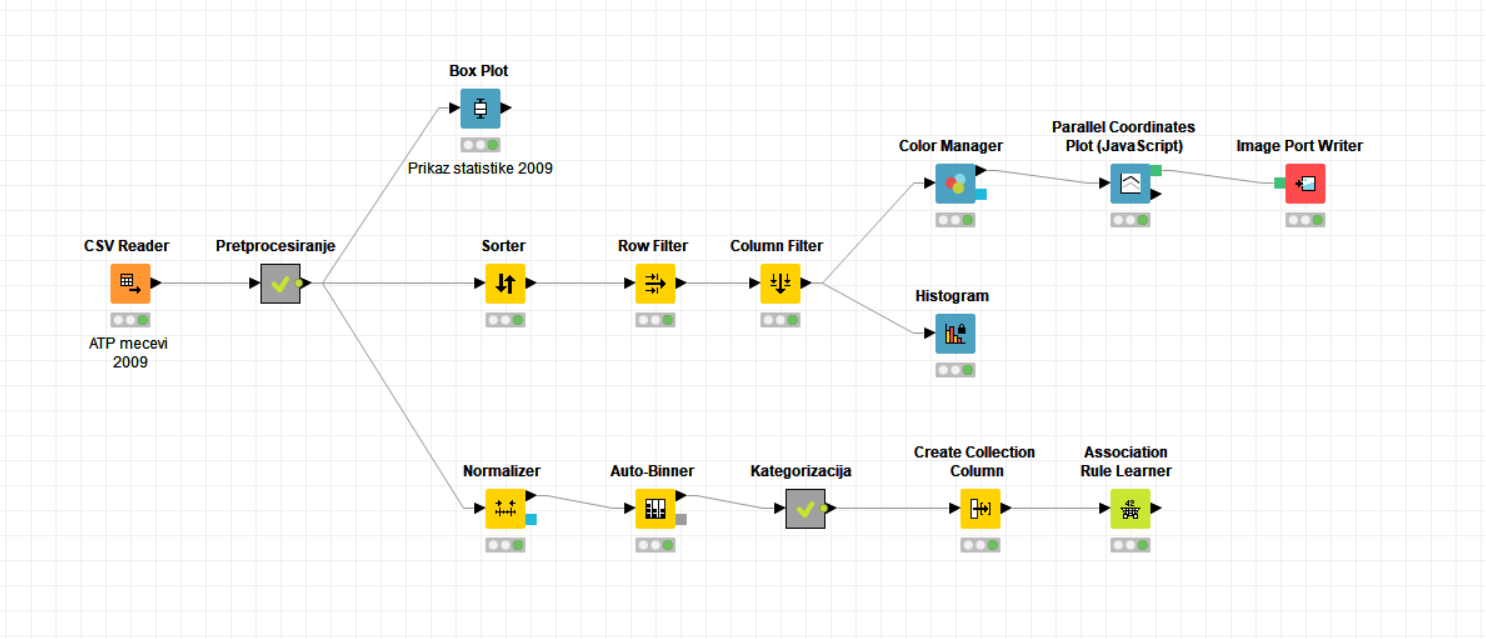
\includegraphics[scale=0.37]{KNIME_project/PravilaPridruzivanja/knime.png}
	\end{center}
	\caption{KNIME implementacija}
	\label{fig:knime}
\end{figure}

Na slikama \ref{fig:histogram} i \ref{fig:parallel} grafički su prikazani rezultati za sedam
tenisera koji su imali prosečno najviše asova po meču na kome su pobedili. Izabrali smo četiri parametra za svakog igrača:
broj asova pobednika, broj dobijenih poena na servis pobednika, broj ubačenih prvih servisa pobednika i
broj osvojenih poena nakon ubačenog prvog servisa pobednika. Na histogramu i grafiku paralelnih koordinata 
mogu se videti i uporediti rezultati.

\begin{figure}[H]
	\begin{center}
		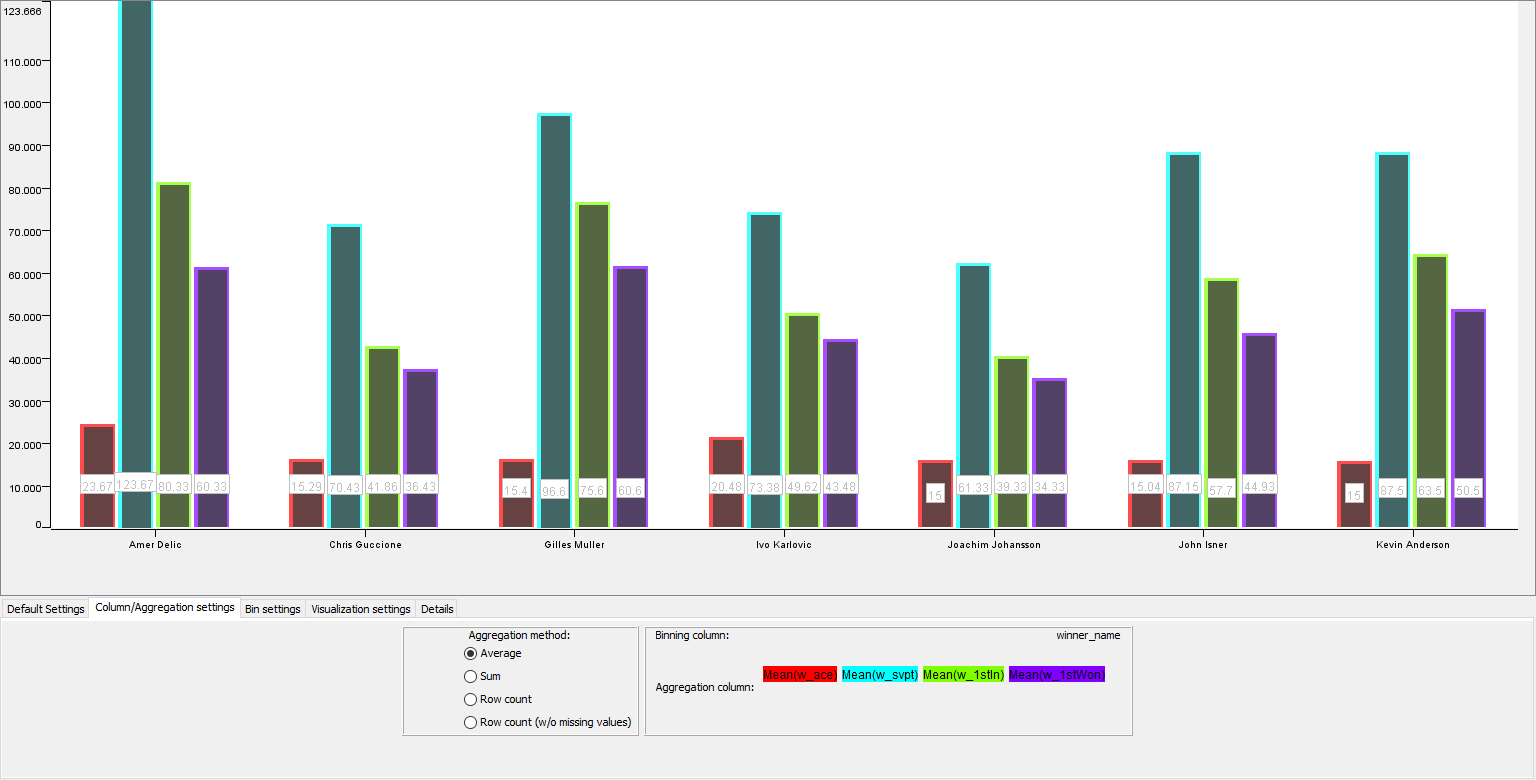
\includegraphics[scale=0.22]{KNIME_project/PravilaPridruzivanja/histogram2009}
	\end{center}
	\caption{Histogram}
	\label{fig:histogram}
\end{figure}

\begin{figure}[H]
	\begin{center}
		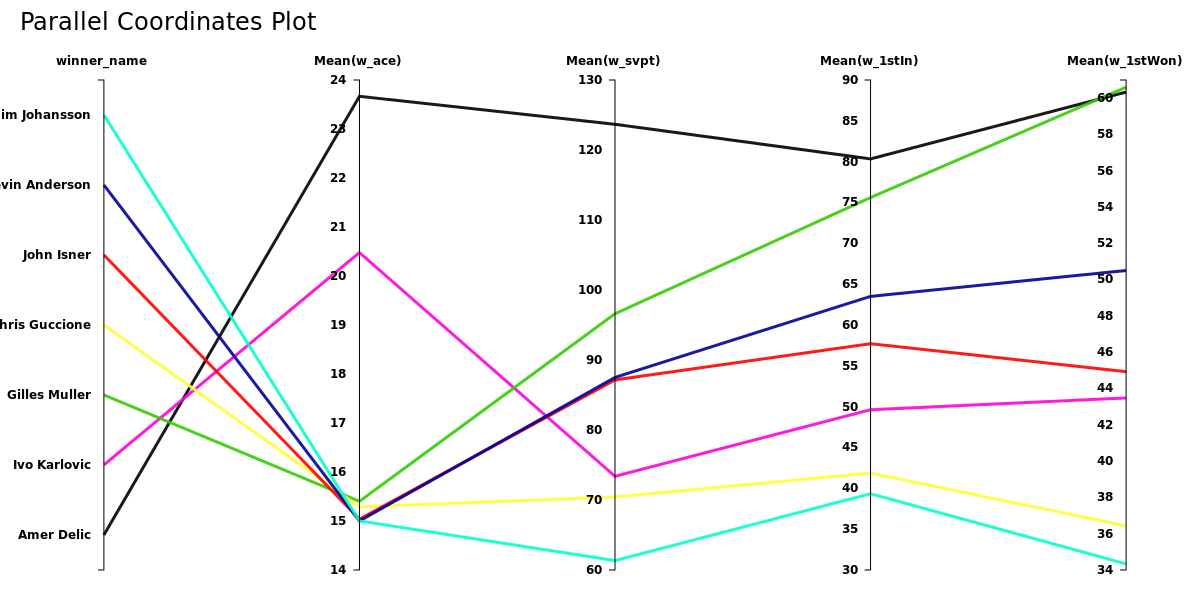
\includegraphics[scale=0.30]{KNIME_project/PravilaPridruzivanja/parallel2009}
	\end{center}
	\caption{Paralelne koordinate}
	\label{fig:parallel}
\end{figure}

Iznenađenje je pojavljivanje Amera Delića u prvih sedam, jer je to
autorima nepoznat igrač. Uvidom u podatke, utvrđeno je da je on te godine odigrao samo osam mečeva,
a pobedio je samo tri puta (što je kriterijum po kome je birano najboljih sedam). \\

U tri kategorije smo podelili sledeća četiri atributa: broj asova pobednika, broj duplih servis grešaka pobednika,
broj osvojenih poena nakon ubačenog prvog servisa pobednika, broj spašenih brejk lopti pobednika.
Na slici \ref{fig:rule_learner} se mogu videti pravila pridruživanja dobijena na osnovu te kategorizacije,
sortirani po Lift meri. Za pouzdanost smo uzeli vrednost 0.4, a za minimalnu podršku vrednost 0.15.
Analizirali smo podatke za sve godine i rezultati su prilično uniformni. Za 2009. godinu je dobijena druga najveća
Lift mera (1.36) i odnosi se na pravilo [ACE 2, WON 2, DF 1] -> [BPS 1].
U 2004. godini smo dobili najveću vrednost Lift mere (1.441) za pravilo [BPS 1, ACE 1, DF 1] -> [WON 1].


\begin{figure}[h!]
	\begin{center}
		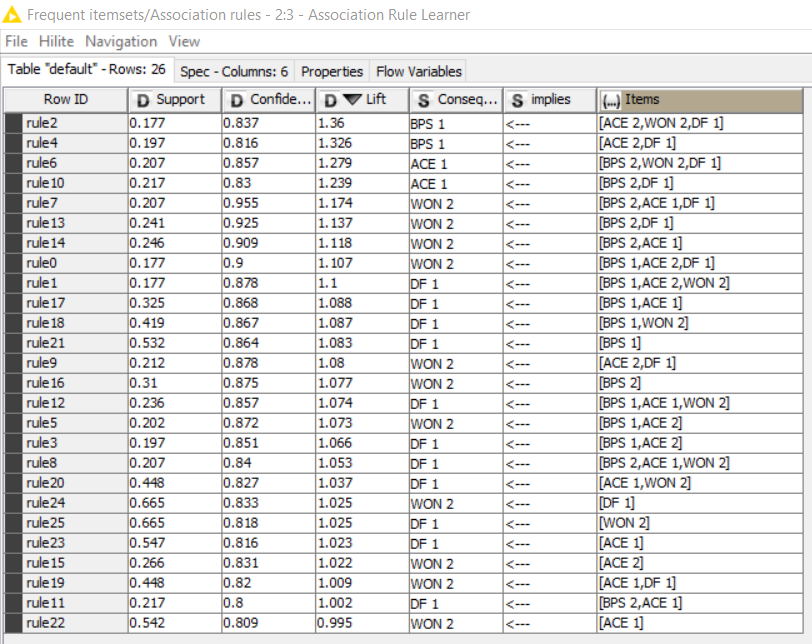
\includegraphics[scale=0.6]{KNIME_project/PravilaPridruzivanja/rule_learner_2009}
	\end{center}
	\caption{Pravila pridruživanja}
	\label{fig:rule_learner}
\end{figure}




\section{Klasterovanje}

\section{Klasifikacija}

\subsection{Klasifikacija u alatu KNIME - SVM}

Klasifikaciju smo vršili na četiri normalizovana atributa: broj asova gubitnika, broj duplih servis grešaka gubitnika,
broj ubačenih prvih servisa gubitnika, broj brejk šansi na servis gubitnika. Ispitivana je zavisnost ovih atributa u odnosu 
na podlogu na kojoj se igra meč.  \\

Vršili smo klasifikaciju tehnikom SVM. Normalizovane podatke smo podelili na trening i test skup u odnosu 70-30.
Primenili smo sva tri raspoloživa kernela (polinomijalni trećeg stepena, sigmoid, Gausov(RBF)).
Na slici \ref{fig:precision} se mogu videti preciznosti za sva tri kernela, i za trening i za test skup.

\begin{figure}[h!]
	\begin{center}
		
\includegraphics[scale=0.42]{KNIME_project/SVM/preciznost}
	\end{center}
	\caption{Preciznost za različite kernele}
	\label{fig:precision}
\end{figure}


Koristeći polinomijalni kernel trećeg stepena, dobili smo izuzetno loše rezultate.
Naime, skoro 50\% redova (1501 od 3257) odgovaraju mečevima koji su odigrani na tvrdoj podlozi.
Na slikama \ref{fig:poly_training} i \ref{fig:poly_test} vidimo da su podaci pogrešno klasifikovani u
mečeve koji su odigrani na šljaci.

\begin{figure}[h!]
	\begin{center}
		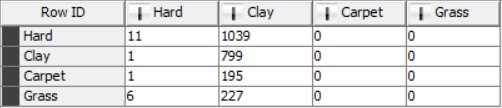
\includegraphics[scale=0.6]{KNIME_project/SVM/poly_training}
	\end{center}
	\caption{Trening podaci za polinomijalni kernel}
	\label{fig:poly_training}
\end{figure}

\begin{figure}[h!]
	\begin{center}
		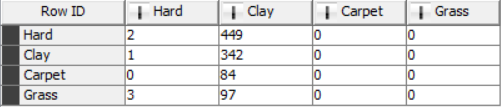
\includegraphics[scale=0.6]{KNIME_project/SVM/poly_test}
	\end{center}
	\caption{Test podaci za polinomijalni kernel}
	\label{fig:poly_test}
\end{figure}

%\newpage

Koristeći sigmoid kernel, situacija se promenila utoliko što su podaci vezani za tvrdu podlogu
vrlo dobro klasifikovani, što se može videti na slikama \ref{fig:sigmoid_training} i \ref{fig:sigmoid_test}.
Primetimo da su podaci uglavnom raspoređeni u klase koje se odnose na beton i šljaku.

\begin{figure}[h!]
	\begin{center}
		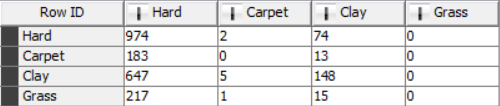
\includegraphics[scale=0.6]{KNIME_project/SVM/sigmoid_training}
	\end{center}
	\caption{Trening podaci za sigmoid kernel}
	\label{fig:sigmoid_training}
\end{figure}

\begin{figure}[h!]
	\begin{center}
		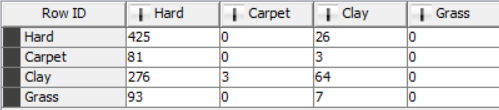
\includegraphics[scale=0.6]{KNIME_project/SVM/sigmoid_test}
	\end{center}
	\caption{Test podaci za sigmoid kernel}
	\label{fig:sigmoid_test}
\end{figure}

Koristeći Gausov kernel, dobili smo lošiju klasifikaciju za tvrdu podlogu, dosta bolju klasifikaciju za šljaku
i malo bolju klasifikaciju za travu (slike \ref{fig:rbf_training} i \ref{fig:rbf_test}). \\

\begin{figure}[h!]
	\begin{center}
		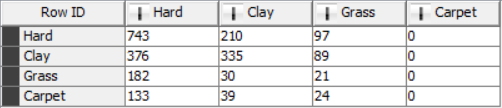
\includegraphics[scale=0.6]{KNIME_project/SVM/rbf_training}
	\end{center}
	\caption{Trening podaci za Gausov kernel}
	\label{fig:rbf_training}
\end{figure}

\begin{figure}[h!]
\begin{center}
	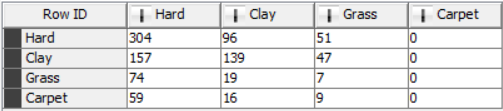
\includegraphics[scale=0.6]{KNIME_project/SVM/rbf_test}
\end{center}
\caption{Test podaci za Gausov kernel}
\label{fig:rbf_test}
\end{figure}

%\newpage

U svim slučajevima, klasifikacija koja se odnosi na tepih je davala nulu. Moguće objašnjenje je činjenica da 10\% podataka
za igranje na tepihu sadrži mnogo kolona sa nedostajućim vrednostima. Potrebna je detaljnija analiza za objašnjenje ovog rezultata klasifikacije,
koja prevazilazi potrebe ovog rada.

	



%Predikat se naziva ekzistencijalan ako se pojavljuje samo u telima pravila (desna strana pravila), inače (ako se pojavljuje bar jednom u glavi pravila) naziva se intenzivan. Skup egzistencijalnih i intenzivnih predikata programa P označava se $ edb(P) $ i $ idb(P) $, respektivno.
%
%%Datalog program P je slojevit ako se njegova pravila mogu podeliti u slojeve $ P\_{1},. . . , P\_{n} $ tako da ako se predikat p pojavio kao pozitivan (negativan) literal u telu pravila u $ P\_{i} $, tada sva pravila sa p u njihovim glavama su u sloju $ P\_{j} $ sa $ j  \leq  i (j  \le  i) $. Slojevitost obezbeđuje da se predikati koji se pojavljuju kao negativni literali u potpunosti definišu u nižim slojevima.
%%
%%Sintaksno proširujemo Datalog sa agregatnim funkcijama kao što su $ min $ i $ max $. 
%%	
%%\textbf{Semantika}. Neka je $  A = \{p(t) \mid t  \subseteq Vals \} $ označava skup svih tačaka (tj. slobodnih promenljivih) atoma. Kompletna rešetka $ (P (A),  \subseteq ,  \bigcap , \bigcup , \emptyset , A) $ delimično oddređuje skup interpretacije $ P(A) $.
%%
%%Data zamena $ \sigma \in  Vars \rightarrow  Vals $ mapira promenljive do na vriednos. Dat atom a, možemo da napišemo $ \sigma(a) $ za atom koji dobijen zamenom
%%promenljive u $ a $ prema $ \sigma $ npr., $ \sigma (p(X)) $ vraća atom $ p (\sigma (X)) $.
%%Operator posledica $ TP \in P(A) \rightarrow P(A) $ za program P je definisan kao:\\
%%
%%	\hspace{1.5cm} $ TP (A) = A \bigcup \{\sigma(a) | a \leftarrow l1. . . ln \in P, \forall li \in l. A \models  \sigma(li)\} $\\
%%	
%%gde je $ A \models \sigma(a) $ ako $ \sigma(a) \in A $ i $ A \models  \sigma(\neg a) $ ako  $ \sigma(a) \in A $.
%%
%%Ulaz za P je skup atoma konstruisan korišćenjem ekzistencijalnih predikata. Neka je P program sa slojevima $ P\_{1},. . . , P\_{n} $ i I biti ulaz za P. Model P za I, označen sa $ [[P]] I $, je $ M\_{n} $, gde je $ M\_{0} = I $ i $  Mi = \bigcap \{A \in fp T\_{Pi} \mid A \subseteq M\_{i-1}\} $ je najmanja fiksna tačka $ T\_{Pi} $ koja je veća od najnižeg sloja modela $ M\_{i-1} $.
%%
%\section{Deklarativna mrežna specifikacija}
%
%U ovom odeljku prvo opisujemo kako definišemo ponašanje mreže kao Datalog program. Nakon toga, raspravljamo o tome kako su uslovi za rutiranje navedeni kao ograničenja preko fiksne tačke programa Datalog.
%
%\subsection{Specifikacija mreža}
%
%Kako bi verno opisali ponašanje mreže, modelujemo:
%\begin{itemize}
%	\item ponašanje protokola rutiranja i njihovih interakcija 
%	\item topologiju mreže.
%\end{itemize}
%
%\textbf{Izražavanje protokola u Datalogu}. Formalizujemo pojedinačne protokole rutiranja i kako ruteri kombinuju sledeće ulaze izračunate ovim protokolima kao Datalog program N. Datalog program N izvodi predikat $ Fwd (TC, Router, NextHop) $, koji predstavlja globalno sledeće stanje mreže. Na slici \ref{fig:picture1} (a), na primer, prikazujemo relevantna pravila koja definišu kako se sledeći ulazi izračunati u OSPF-u kombinuju sa onima definisanim putem statičkih ruta. Predikat $ Route(TC, Router, NextHop, Proto) $ snima sledeće ulaze OSPF-a i statičkih ruta. Glavno Datalog pravilo navodi da ruteri biraju, za svaku klasu saobraćaja TC, sledeći ulaz sa minimalnim administrativnim troškovima (minAD) koji se računa po svim protokolima putem drugog Datalog pravila na slici \ref{fig:picture1}(a). Donja dva pravila definišu predikatsku Route, koja prikuplja sledeće ulaze definisane preko statičkih ruta i izračunatih od strane OSPF-a. Napominjemo da su OSPF rute (predstavljene od strane predikata BestOSPFRoute) definisane dodatnim pravilima Datalog-a koja zauzima ponašanje OSPF protokola.
%
%\textbf{Topologija mreže}. Topologija mreže se takođe preuzima preko Datalog pravila u programu N. Modelujemo svaki ruter kao konstantu i koristimo predikate da  predstavljaju topologiju. Na primer, predikat $ SetLink (R1, R2) $ predstavlja da su dva rutera $ R1 $ i $ R2 $ povezana preko puta, i dodajemo pravilo Datalog $ SetLink (R1, R2) \leftarrow true $ koje definiše ovakav put.
%
%\subsection{Određivanje zahteva}
%
%Određujemo zahteve kao ograničenja prvog reda  bez funkcije u odnosu na predikat Fwd (TC, Router, NextHop), koji definiše sledeće stanje mreže. Pišemo $ A \models \phi $ da označimo da Datalog interperetacija $ A $ zadovoljava $ \phi $. Za ilustraciju, opisujemo kako se mogu navesti uobičajeni zahtevi za rutiranje:
%
%	$ Path(TC, R\_{1}, [R\_{1}, R\_{2},..., R\_{n}]) $ (Zahtev putanje): paketi za TC klasu saobraćaja moraju da prate put $ R\_{1}, ..., R\_{n} $. Ovi zahtevi su navedeni kao konjunkcija nad predikatom Fwd.
%	
%	$ \forall R\_{1}, R\_{2}. Fwd(TC1, R1, R2) \Rightarrow \neg Fwd(TC2, R1, R2) $ (Izolacija saobraćaja): putanja za dve različite klase saobraćaja TC1 i TC2 ne dele put u istom pravcu. 
%
%	$ Reach(TC, R\_{1}, R\_{2}) $ (Dostupnost): paketi za TC klasu saobraćaja mogu da dosegnu ruter R2 od rutera R1. Predikat $ Reach $ predstavlja tranzitivno zatvaranje predikata $ Fwd $ (definisanog preko Datalog pravila).
%	
%	$ \forall TC, R . (\neg Reach(TC, R, R))$ (Petlja bez): generički zahtev propisuje da sledeća oblast nema petlje.
%
%Složeniji zahtevi, kao što je način upućivanja, mogu se navesti na osnovu ograničenja prvog reda bez funkcija koje pruža SyNET. Dalje, SyNET se može koristiti kao bekend za jezik visokog nivoakoji je lakši za korišćenje od strane mrežnog operatera.
%
%\subsection{Konfiguracija mreže}
%
%Konfiguracije ulaznih protokola raspoređene na mrežnim ruterima su predstavljenje kao ulazni \textit{edb} predikat za Datalog programe koji formalizuju
%protokole. Na primer, lokalna konfiguracija OSPF-a za ruter određuje težine puta povezanih sa tim ruterom. Ovo je predstavljeno od \textit{edb} predikata $ SetOSPFEdgeCost (Router, NextHop, Veight) $.
%
%Podskup sintetizovanog Datalog ulaza za naš motivacioni primjer je dati na slici \ref{fig:picture1}(d). Ovde \textit{SetAD} definiše administrativne troškove statičkih ruta da budu niži od onog kod OSPF-a (tako da su statični putevi preferiraniji nego sledeći ulaz računat za OSPF). Predikat $ SetStatic (N\_{1}, A, B) $, koji definiše statičku rutu za $ N\_{1} $ od A do B. Predikat $ SetOSPFEdgeCost $ definiše težine putanja.
%
%\section{Sinteza ulaza za Datalog}
%
%Sada predstavljamo novi iterativni algoritam sinteze ulaza za Datalog. Prvo opisujemo \textit{tok visokog nivoa} algoritma pre nego što pređemo na detalje.\\
%
%\textbf{Tok visokog nivoa}. Razmotrite Datalog program sa slojevima $ P\_{1} $, $ P\_{2} $, i $ P\_{3} $, prikazano na Slici \ref{fig:picture3}. Ulazni i izlazni čvorovi sloja $ P\_{i} $ ukazuju da su $ edb $ predikati i,  $ idb $ predikati tog sloja. Na primer, sloj $ P\_{3} $ uzima kao ulaz predikat $ q(\bar{t}) $ i $ r(\bar{t}) $ i izvodi predikat $ s(\bar{t}) $. Naš iterativni algoritam prvo sintetiše ulaz $ I\_{3} $ za $ P\_{3} $ koje određuje predikati $ q(\bar{t}) $ i $ r(\bar{t}) $ tako da $ P1 \bigcup P2 $ izlazi. Da bi sintetisali takav ulaz za jedan sloj, predstavljamo algoritam koji se zove \textbf{$ S\_{SemiPos} $}, koji se bavi problemom sinteze ulaza za polu-pozitivni Datalog programi, tj. Datalog programe u kojima je negiranje ograničeno $ edb $ predikatima. Nakon sinteze ulaza $ I\_{3} $ za $ P\_{3} $, naš iterativni algoritam sintetiše ulaz $ I\_{2} $ za $ P\_{2} $ tako da fiksna tačka $ [[P\_{2}]] I\_{2} $ proizvodi predikate $ r(\bar{t}) $ koji se nalaze u već sintetizovanom ulazu $ I\_{3} $ za $ P\_{3} $. Napominjemo da ovakav iterativni proces može zahtevati bektreking, u slučaju da nema ulaza za $ P\_{2} $ može se proizvesti željeni predikat $ r(\bar{t}) $ sadržani u $ I\_{3} $. Algoritam se prekida kada sintetiše ulazne podatke za sva tri sloja.
%
%\begin{figure}[h!]
%	\begin{center}
%		\includegraphics[scale=0.50]{resources/picture3.png}
%	\end{center}
%	\caption{Datalog program sa slojevima P1, P2 i P3, i protokom predikata između slojeva.}
%	\label{fig:picture3}
%\end{figure}
%
%U nastavku, prvo predstavljamo algoritam \textbf{$ S\_{SemiPos} $} koji se koristi da se izvrši sinteza ulaza za jedan sloj (što je polu-pozitivan program). Zatim predstavljamo opšti algoritam, nazvan \textbf{$ S\_{Strat} $}, koji iterativno primjenjuje $ S\_{SemiPos} $ za svaki sloj koji sintetiše ulaze za Datalog programe.
%
%\subsection{Sinteza ulaza za polu-pozitivan Datalog sa SMT-om}
%
%Ključna ideja je da se problem sinteze ulaza svede na zadovoljavanje SMT ograničenja: Dat je polu-pozitivan Datalog program P i ograničenje $ \phi $, kodiramo $ \exists I . [[P]] I \models \phi $ u SMT ograničenju $ \psi $. Ako je $ \psi $ zadovoljavajuće, onda iz modela $ \psi $ možemo izvući ulaz I takav da $ [[P]] I \models \phi $.
%
%\begin{figure}[h!]
%	\begin{center}
%		\includegraphics[scale=0.50]{resources/SemiPos.png}
%	\end{center}
%\end{figure}
%
%Algoritam $ S\_{SemiPos}(P,\phi) $, dat u algoritmu 1, prvo se poziva funkcija $ Simplify(\phi) $ koja:
%\begin{itemize}
%	\item instancira bilo koji kvantifikator u $ \phi $
%	\item transformiše rezultat u konjukciju klauzula, gde je svaka klauzula disjunkcija literala
%\end{itemize}
%
%Zatim, algoritam iterativno odvija Datalog pravila, do unapred zadate granice, nazvane $ bound\_{k} $. U svakom koraku for-petlje, algoritam generiše SMT ograničenje koje obuhvata:
%	\begin{itemize}
%		\item koji atomi se izvedu nakon k primena P pravila
%		\item koji atomi nikad nisu izvedeni od strane P-a.
%	\end{itemize} 
%SMT ograničenje označeno je sa $ [P]\_{k} $. Algoritam takođe prepisuje pojednostavljeno ograničenje $ \phi\prime $ koristeći funkciju $ Rewrite (\phi\prime, k) $ koja rekurzivno prolazi konjunkcije i disjunkcije u pojednostavljenom ograničenju $ \phi\prime $ i mapira pozitivne literale na
%predikat $ p\_{k}(t) $ i negativne literale na $ \neg p(t) $:
%
%\begin{figure}[h!]
%	\begin{center}
%		\includegraphics[scale=0.50]{resources/SemiPos1.png}
%	\end{center}
%\end{figure}
%
%Ako je ograničenje $ [P]\_{k} \bigwedge \phi\_{k} $ zadovoljivo, onda je ulaz izveden projekcijom interpretacije I koja zadovoljava ograničenje svih predikata $ edb(P) $. Takođe ako postoji ulaz I takav da je $ [[P]] I \models \phi $ i za koji je fiksirana tačka $ [[P]] I $ dostigla manje od graničnih koraka, onda $ S\_{SemiPos}(P,\phi) $ zagarantovano vraća ulaz.
%
%%Note that since ∨ and ∧ are monotone, negative literals constitute negative
%%constraints and positive literals constitute positive constraints.
%%If the resulting constraint [P ]k ∧ ψk is satisfiable, then an input is derived by projecting the interpretation I that satisfies the constraint over all edb predicates. Note that if there is an input I such that [[P ]]I |= φ and for which the fixed point [[P ]]I is reached in less than boundk steps, then SSemiP os (P, φ) is guaranteed to return an input.
%
%\subsection{Iterativna sinteza ulaza za Datalog}
%
%\begin{figure}[h!]
%	\begin{center}
%		\includegraphics[scale=0.50]{resources/Strat.png}
%	\end{center}
%\end{figure}
%
%Prikaz algoritma dat je na Slici \ref{fig:strat}. Pretpostavimo bez gubitka opštosti da je ograničenje fiksne tačke $ \phi $ definisano preko predikata koje se pojavljuju u najvišem sloju $ P\_{n} $. Počevši od najvišeg sloja $ P\_{n} $, $ S\_{Strat} $ generiše ulaz $ I\_{n} $ za $ P\_{n} $ tako da $ [[P\_{n}]] I\_{n} \models \phi $. Zatim se iterativno sintetiše ulaz za donje slojeve $ P\_{n-1},. . . , P\_{1} $ koristeći algoritam $ S\_{SemiPos} $. Na kraju, da bi se konstruisao ulaz za P, algoritam kombiniju ulaze sintetizovane za sve slojeve i vraća ulaz I za P.
%
%\section{Implementacija i procena}
%
%U ovom odeljku predstavljen je SyNET, i krajnja implementacija algoritma sinteze ulaza koji se primjenjuje na mrežni problem sinteze. Zatim se okrećemo oceni SyNET-a na praktičnim topologijama i zahtevima.
%
%\subsection{Implementacija}
%
%SyNET je implementiran u Python-u i automatski kodira Datalog programe u SMT ograničenjima. Koristi Python API da bi proverio da li su generisana SMT ograničenja zadovoljavajuća i da dobije model.
%
%SyNET podržava rutere koji pokreću oba, OSPF i BGP protokola i koji se mogu konfigurisati statičkim rutama. SyNET koristi prirodno razdvajanje protokola:
%spoljašnje putanje obavlja BGP, dok unutrašnjim rukuju IGP protokoli (OSPF sa statičkim rutama). Pravila Dataloga koja obuhvataju ove protokole i njihove zavisnosti podeljenja su u 8 slojeva. Za većinu topologija i zahteva, Datalog program dostigne fiksnu tačku u roku od 20 iteracija, pa smo fiksirali granice za odvijanje i bektreking na 20.
%
%Jednostavna skripta se može koristiti za konvertovanje izlaza iz SzNET-a u bilo koji specifični konfiguracioni format, a zatim ih razviti u rutere. Zaista, za testiranje ispravnosti SyNET-a, primenjuje se mala skriptu za pretvaranje unosa sintetizovanog od strane SyNET-a do Cisco ruter konfiguracije.
%
%SyNET podržava dve ključne optimizacije koje poboljšavaju performanse. Prva optimizacija je parcijalna evaluacija: SyNET delimično procenjuje pravila Dataloga sa
%predikatima čije su istinitosne vrednosti poznate \textit{a priori}. Druga optimizacija predstavlja ograničenja specifična za mrežu: konfigurisali smo SyNET sa generičkim ograničenjima, koja su tačna za sva sledeća stanja, i sa ograničenjima koja se održavaju za bilo koji ulaz u određeni protokol. 
%
%\subsection{Eksperimenti}
%
%%To investigate SyNET’s performance and scalability, we experimented with differ-
%%ent: (i) topologies, (ii) requirements; and (iii) protocol combinations. Further to
%%test correctness, we ran all synthesized configurations on an emulated environ-
%%ment of Cisco routers [32] and we verified that the forwarding paths computed
%%match the requirements for each experiment.
%
%Kako bismo istražili performanse i skalabilnost SyNET-a, eksperimentirali smo sa različitim:
%\begin{itemize}
%	\item topologijama
%	\item zahtevima
%	\item kombinacijom protokola.
%\end{itemize} 
%Dalje za ispravnost testova, pokreću se sve sintetizovane konfiguracije u simuliranom okruženju Cisco rutera i proverava se da sledeći putevi odgovaraju zahtevima za svaki eksperiment.
%
%%Network Topologies. We used network topologies that have between 4 and
%%64 routers. The 4-router network is our overview example where we considered
%%the same requirements as those described in Sect. 2. The 9-router network is
%%Internet2 (see Fig. 5), a US-based network that connects several major universi-
%%ties and research institutes. The remaining networks are n x n grids.
%
%\textbf{Topologija mreže} Koristili smo topologiju mreže koja ima između 4 i 64 rutera. Mreža sa 4 rutera je naš primer opisana u Sekt. 2. Mreža sa 9 rutera je
%Internet2 (vidi sliku 5), mreža zasnovana na SAD-u koja povezuje nekoliko glavnih univerziteta i istraživačkih instituta. Preostale mreže su $ n \times n $ mreže.
%
%%Routing Requirements. For each router and each traffic class, we generate
%%a routing requirement that defines where the packets for that traffic class must
%%be forwarded to. We consider 1, 5, and 10 traffic classes. For a topology withrouters and m traffic classes, we thus generate n x m requirements.
%
%\textbf{Zahtevi rutiranja} Za svaki ruter i svaku klasu saobraćaja generišemo zahtev za usmeravanje koje definiše gde paket za tu klasu saobraćaja mora biti proslijeđen. Razmatramo 1, 5 i 10 klasa saobraćaja. Za topologiju sa ruterima i m klasa saobraćaja, generišemo $ n \times m $ zahteve.
%
%%For topologies with multiple traffic classes, we add one external network
%%announced by two randomly selected routers. We add requirements to enforce
%%that all packets destined to the external networks are forwarded to one of the
%%two routers. This models a scenario where the operator is planning maintenance
%%downtime for one of the two routers. Further, to show that SyNET synthesizes
%%configurations with partially defined input and protocol dependencies, we assume
%%the local BGP preferences are fixed by the network operator and thus SyNET has
%%to synthesize correct OSPF costs to meet the BGP requirements.
%
%Za topologije sa više klasa prometa, dodamo jednu spoljnu mrežu napravljenu od strane dva slučajno izabrana rutera. Dodamo zahteve da svi paketi namenjeni spoljnim mrežama budu prosleđeni jednom od dva rutera. Ovi modeli predstavljaju scenario gde operater planira održavanje za jedan od dva rutera. Dalje, kako bi se pokazalo da SyNET sintetizuje konfiguracije sa delimično definisanim zavisnim ulazima i protokolima, pretpostavljamo da su lokalne pretpostavke BGP-a fiksirane od strane operatora mreže i na taj način SyNET može da sintetiše tačne OSPF troškove kako bi ispunio BGP zahteve.
%
%%Protocols. We consider three different combinations of protocols: (i) static routes; (ii)
%%OSPF and static routes; and (iii) OSPF, BGP, and static routes. The protocol combinations (i) and (ii) ignore requirements for
%%external networks since only BGP computes routes for them.
%
%\textbf{Protokoli} Razmatramo tri različite kombinacije protokola: 
%	\begin{enumerate}
%		\item statički putevi
%		\item OSPF i statički putevi
%		\item OSPF, BGP i statički putevi
%	\end{enumerate}
%Kombinacije protokola 1) i 2) ignorišu zahteve za spoljne mreže, jer jedini BGP obračunava puteve za njih.

\end{document}
